
Once the Raa for the $\PgUc$ signal is extracted from the simultaneous ML fit, 
we employ the Feldman-Cousins (FC) prescription to set a limit at $95\%$ confidence level~\cite{MCMC}. 
While the expected limit on the nuclear modification factor is close to a
 non-physical ($\leq 0$) result, %(i.e. $\raa(\PgUc) \leq  0$), 
the FC prescription guarantees a physically meaningful result and tells us how to smoothly 
transition from one-sided to two-sided limit. 
%The FC prescription is described in detail in Ref.~\cite{FC}. % Ref missing!
It uses a likelihood ratio as an ordering principle for selecting the acceptance
 region and creating confidence bands. The likelihood ratio is defined as the following:
\begin{equation}
Q(x)=\frac{P(x|\raa(\PgUc)_{0})}{P(x|\raa(\PgUc)_{\text{max}})} \,,
\end{equation}
where $Q(x)$ is a likelihood ratio for given $\raa(\PgUc)$, x,  a given $\raa(\PgUc)$ and finally $\raa(\PgUc)_{0}$,
and $\raa(\PgUc)_{\text{max}}$ is the $\raa(\PgUc)$ for the maximum likelihood among all possible $\raa(\PgUc)$ values.


%\subsubsection{Nuclear modification factor upper limit}
%\label{sec:raa_limits}

For the centrality-integrated bin (0 -100\%) the computed upper limit for the nuclear modification factor, $\raa(\PgUc)$, using the FC method is about 0.095 (95\% CL). This can be seen from \fig{fig:FC_Raa_Limit_MB}, when the observed $CL_s$ (red dots) crosses the horizontal threshold (red line). We generate 1000 pseudo experiments at each scanned point to discriminate the null hypothesis (no signal 3S is present) from the alternative (signal plus background) hypothesis.
%Results are summarized in Table.~\ref{tab:Raaupperlimits}. 

\begin{figure}[hbtp]
  \begin{center}
   %\subfigure[$p$-value scan using Feldman Cousins technique]{
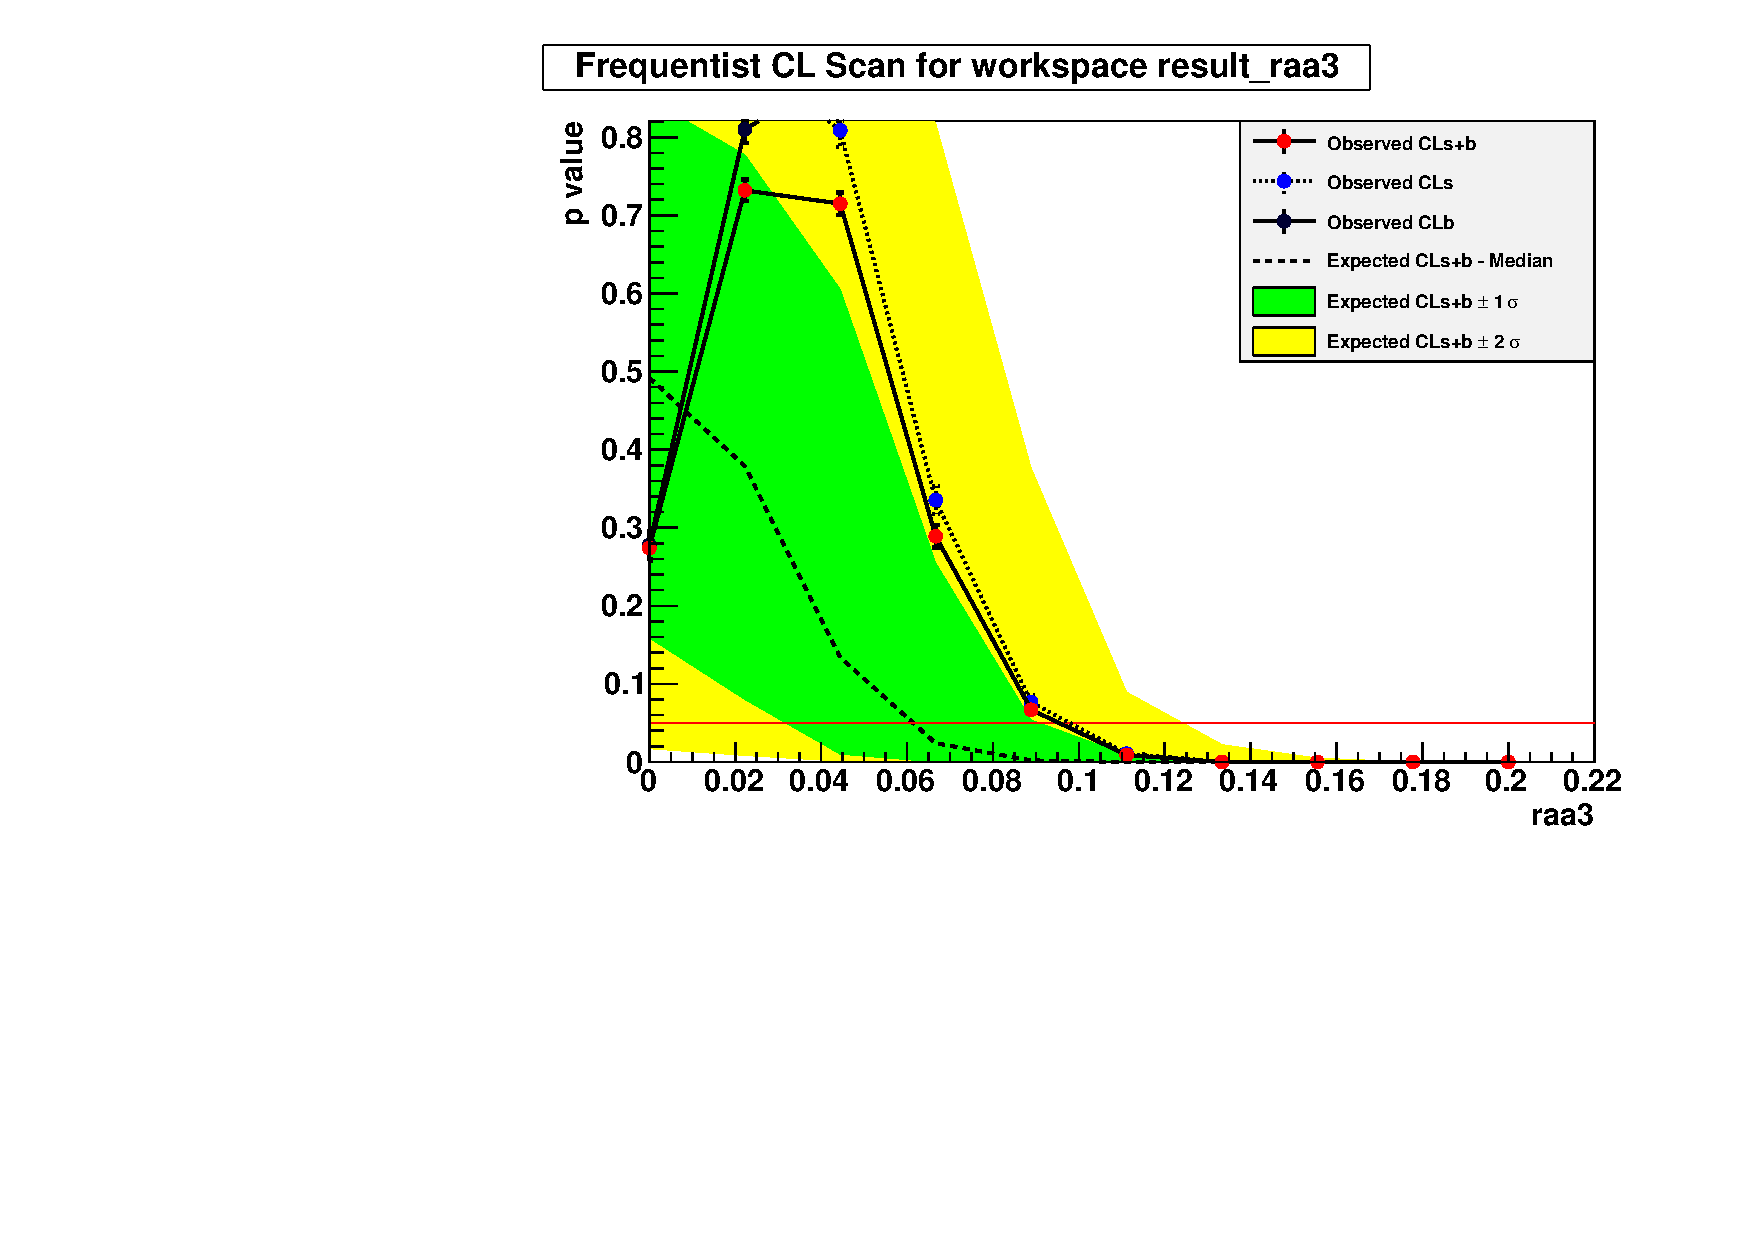
\includegraphics[angle=0,width=0.7\textwidth]{figures/limits//FC_Raa_Limit_MB}\label{fig:/FC_Raa_Limit_MB}
%}\\
   \caption{$p$-value scan for $\raa(\PgUc)$ using the Feldman-Cousins technique.}
%A thousand pseudo experiments for each of the ten points scanned. Figs~\ref{fig:/FC_Raa_Limit_MB}:Observed $CL_s$; red curve, $H_{b}$ blue curve and black line is our Test Statistics.}
   \label{fig:FC_Raa_Limit_MB}
 \end{center}
\end{figure}

\begin{figure}[hbtp]
  \begin{center}
   \subfigure[Pseudo-experiments for null and alternative hypotheses and using likelihood ratio test statistics.]{
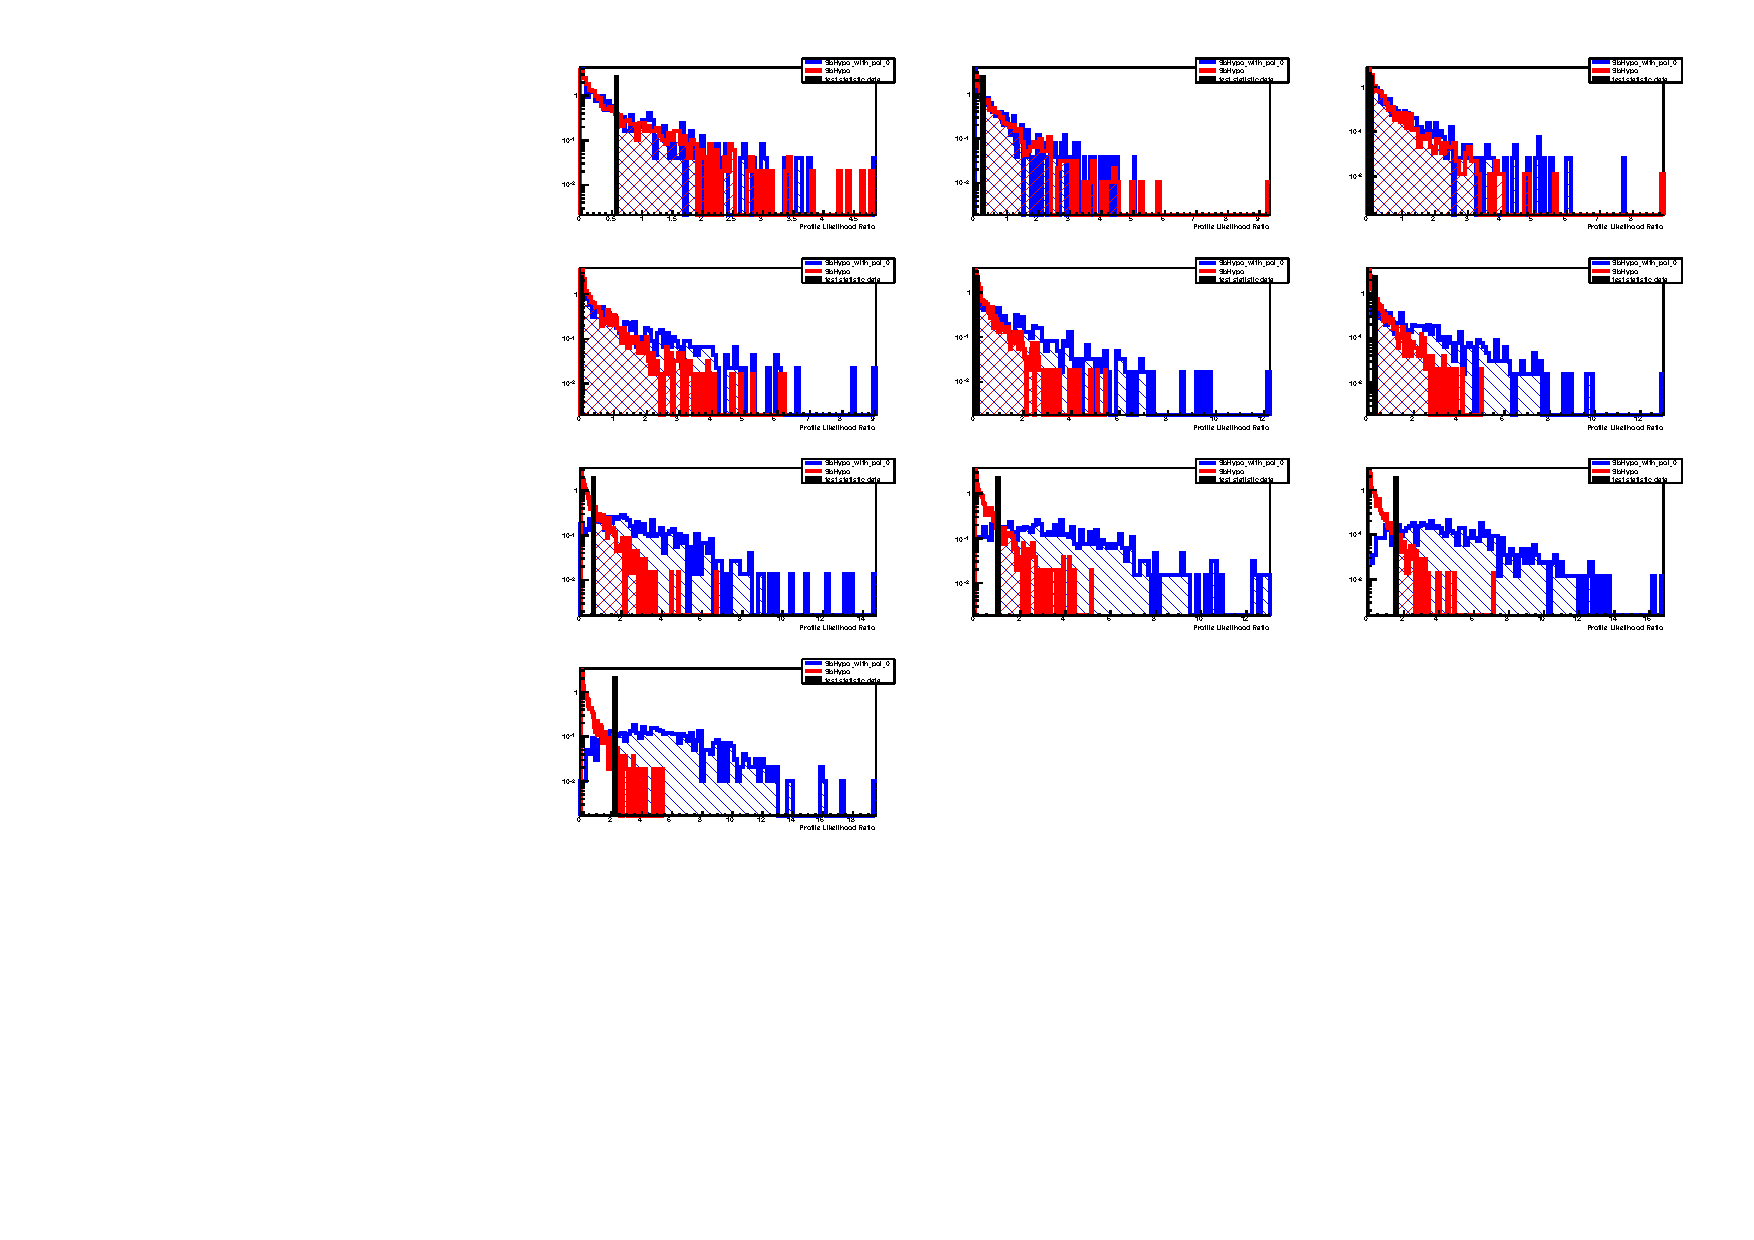
\includegraphics[angle=0,width=1.0\textwidth]{figures/limits//FCRaa3SToyswithSystematics}\label{fig:/FCRaa3SToyswithSystematics}}\\
   \caption{A thousand pseudo-experiments for each of the ten points scanned. %Figs~\ref{fig:/FCRaa3SToyswithSystematics}: 
$H_{sb}$; red curve, $H_{b}$ blue curve and black line is the test statistic. As we increase our parameter of interest it is easier to differentiate between the two hypotheses and the area under the red curve becomes smaller than the area under the blue curve.}
   \label{fig:Raatoys}
 \end{center}
\end{figure}

%\subsection{Propagation of systematic uncertainties on the limits}
%\label{sec:sysRaa}

%Because we use the reconstructed dimuon mass distributions to extract the upsilon $\raa(\PgUc)$,
%any systematic that possibly alters the shape and location of the reconstructed
%$\PgU$ mass distributions will potentially change the fitted  \raa\ out of the
%likelihood fitter. 

%\par 
The systematics uncertainties on the \pp luminosity, the nuclear overlap function $\taa$ and the efficiency ratios as well as the uncertainties for the background shape and the signal FSR need to be taken into consideration when setting the upper limit. We fold in these systematics, which were previously specified, via nuisance parameters in the fit.  
%Variation of such parameters corresponds to certain systematic uncertainties. %?..


Figure~\ref{fig:plr_Raa3S_withSystematics} %%Figure 35 %FIXME!!!!!! 
shows cross checks using the profile likelihood ratio implementation, where an $\raa(\PgUc)$ upper limit of about 0.0952 (95\% CL) is obtained. 
Notice that both results are consistent within uncertainties.  
The results for the two implementations are summarized in Table~\ref{tab:Raaupperlimits}.  

\begin{figure}[hbtp]
  \begin{center}
  % \subfigure[Pseudo Experiments for null and alternative hypotheses and using likelihood ratio test statistics]{
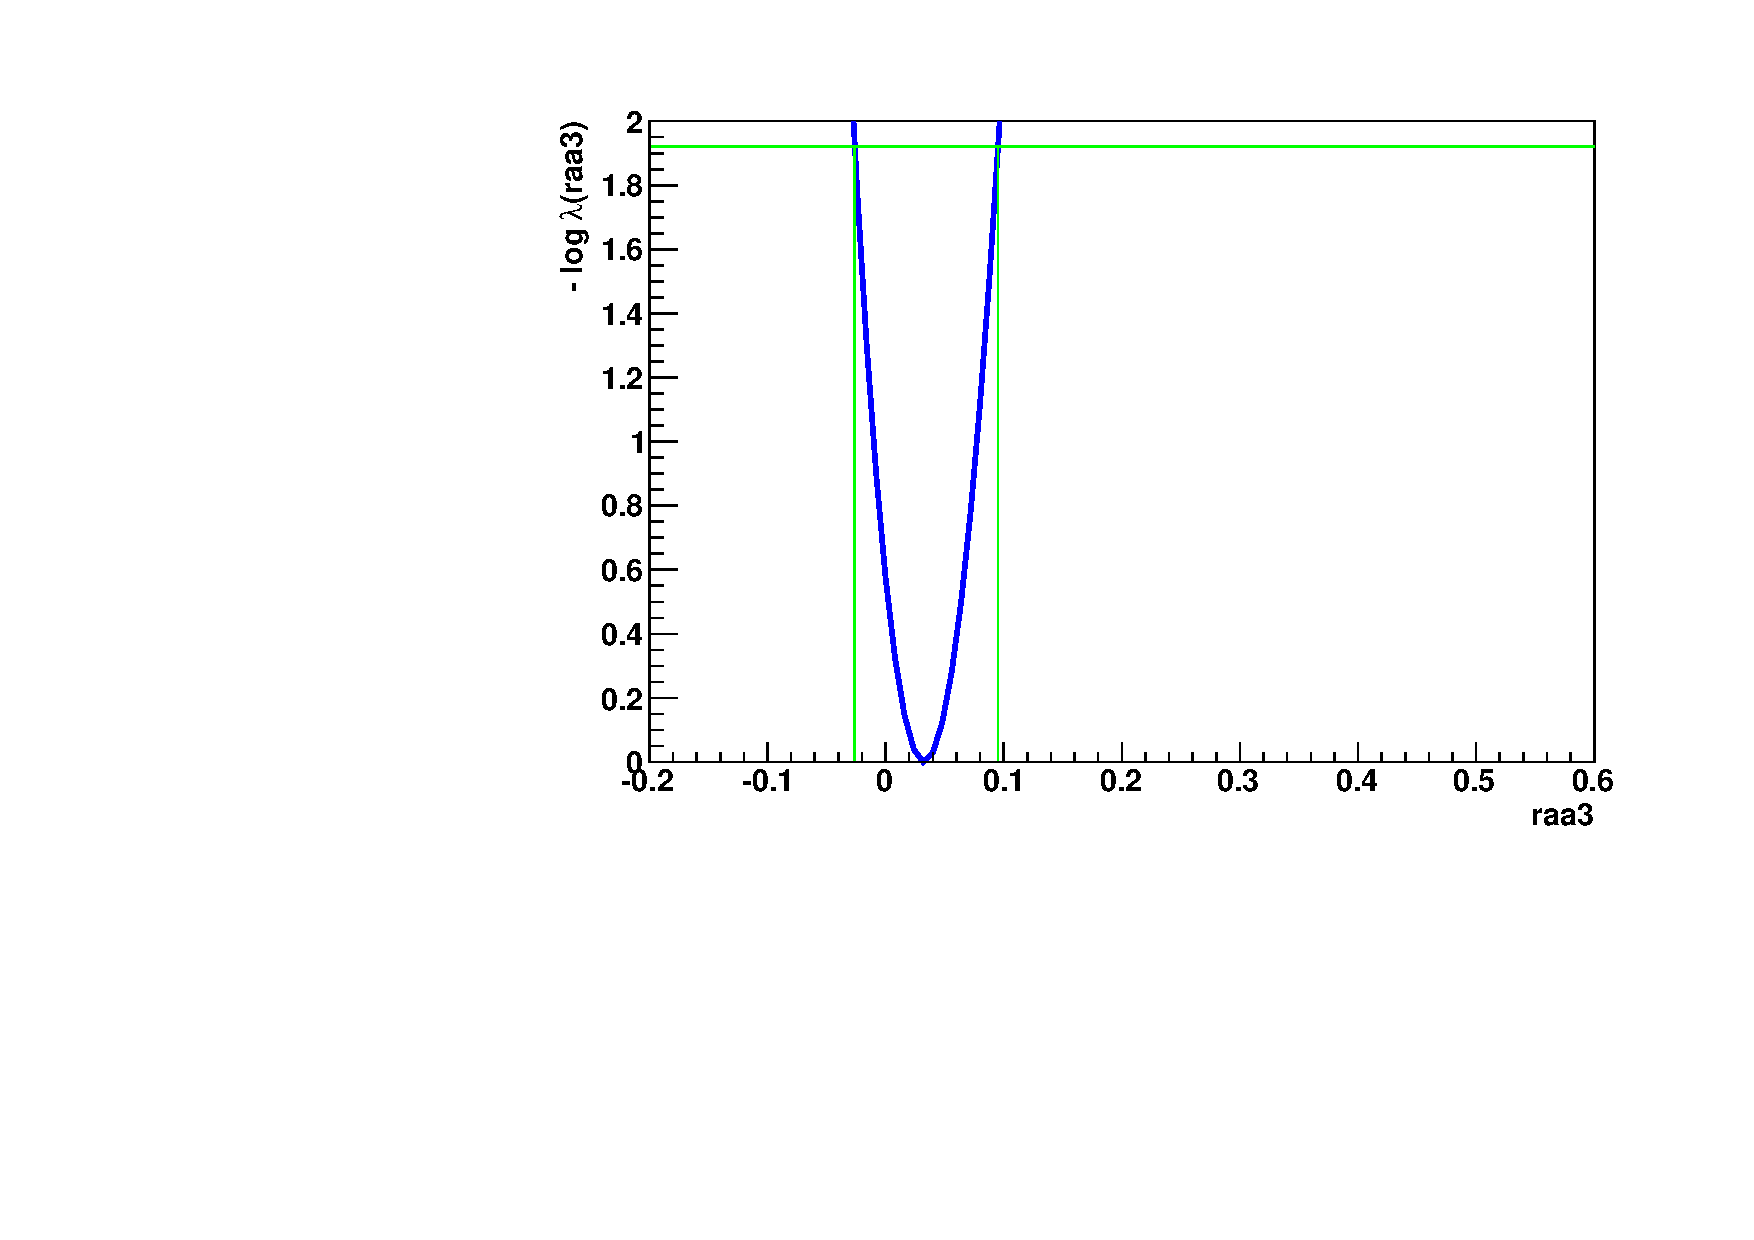
\includegraphics[angle=0,width=0.7\textwidth]{figures/limits//plr_Raa3S_withSystematics}\label{fig:/plr_Raa3S_withSystematics}
%}\\
   \caption{Profiled likelihood ratio. %Figs~\ref{fig:/plr_Raa3S_withSystematics}: 
It shows the confidence interval at $95\%$ confidence level.}
   \label{fig:plr_Raa3S_withSystematics}
 \end{center}
\end{figure}


 
\begin{table}[!v]
  \centering
  \caption{$\raa(\PgUc)$ upper limits. \emph{(Note: being updated)}}
  \begin{tabular}{c|c|c|c}
    \hline
    & & \multicolumn{2}{c}{95\% C.L upper limit}  \\
    centrality & best fit value & Feldman-Cousins & profile likelihood ratio  \\
    \hline
    0 - 100\% & $ 0.032 \pm  0.031$ &$ 0.09506 \pm 0.00130$ & $0.0952$ \\
    \hline
  \end{tabular}
  \label{tab:Raaupperlimits}
\end{table}

Since we are interested in the suppression pattern of the three $\Upsilon$ states and because the errors for the Raa for the $\Upsilon(1S)$ and $\Upsilon(2S)$ have been calculated with a 1 $\sigma$ error, we also set the upper limits at a 68\% confidence level.

In this scenario the upper limit using the Feldman Cousins technique is 

$\raa(\PgUc) \leq 0.064 \pm 0.001$  at 68\% confidence level.



\begin{figure}[hbtp]
  \begin{center}
   %\subfigure[$p$-value scan using Feldman Cousins technique at 68\% confidence level]{
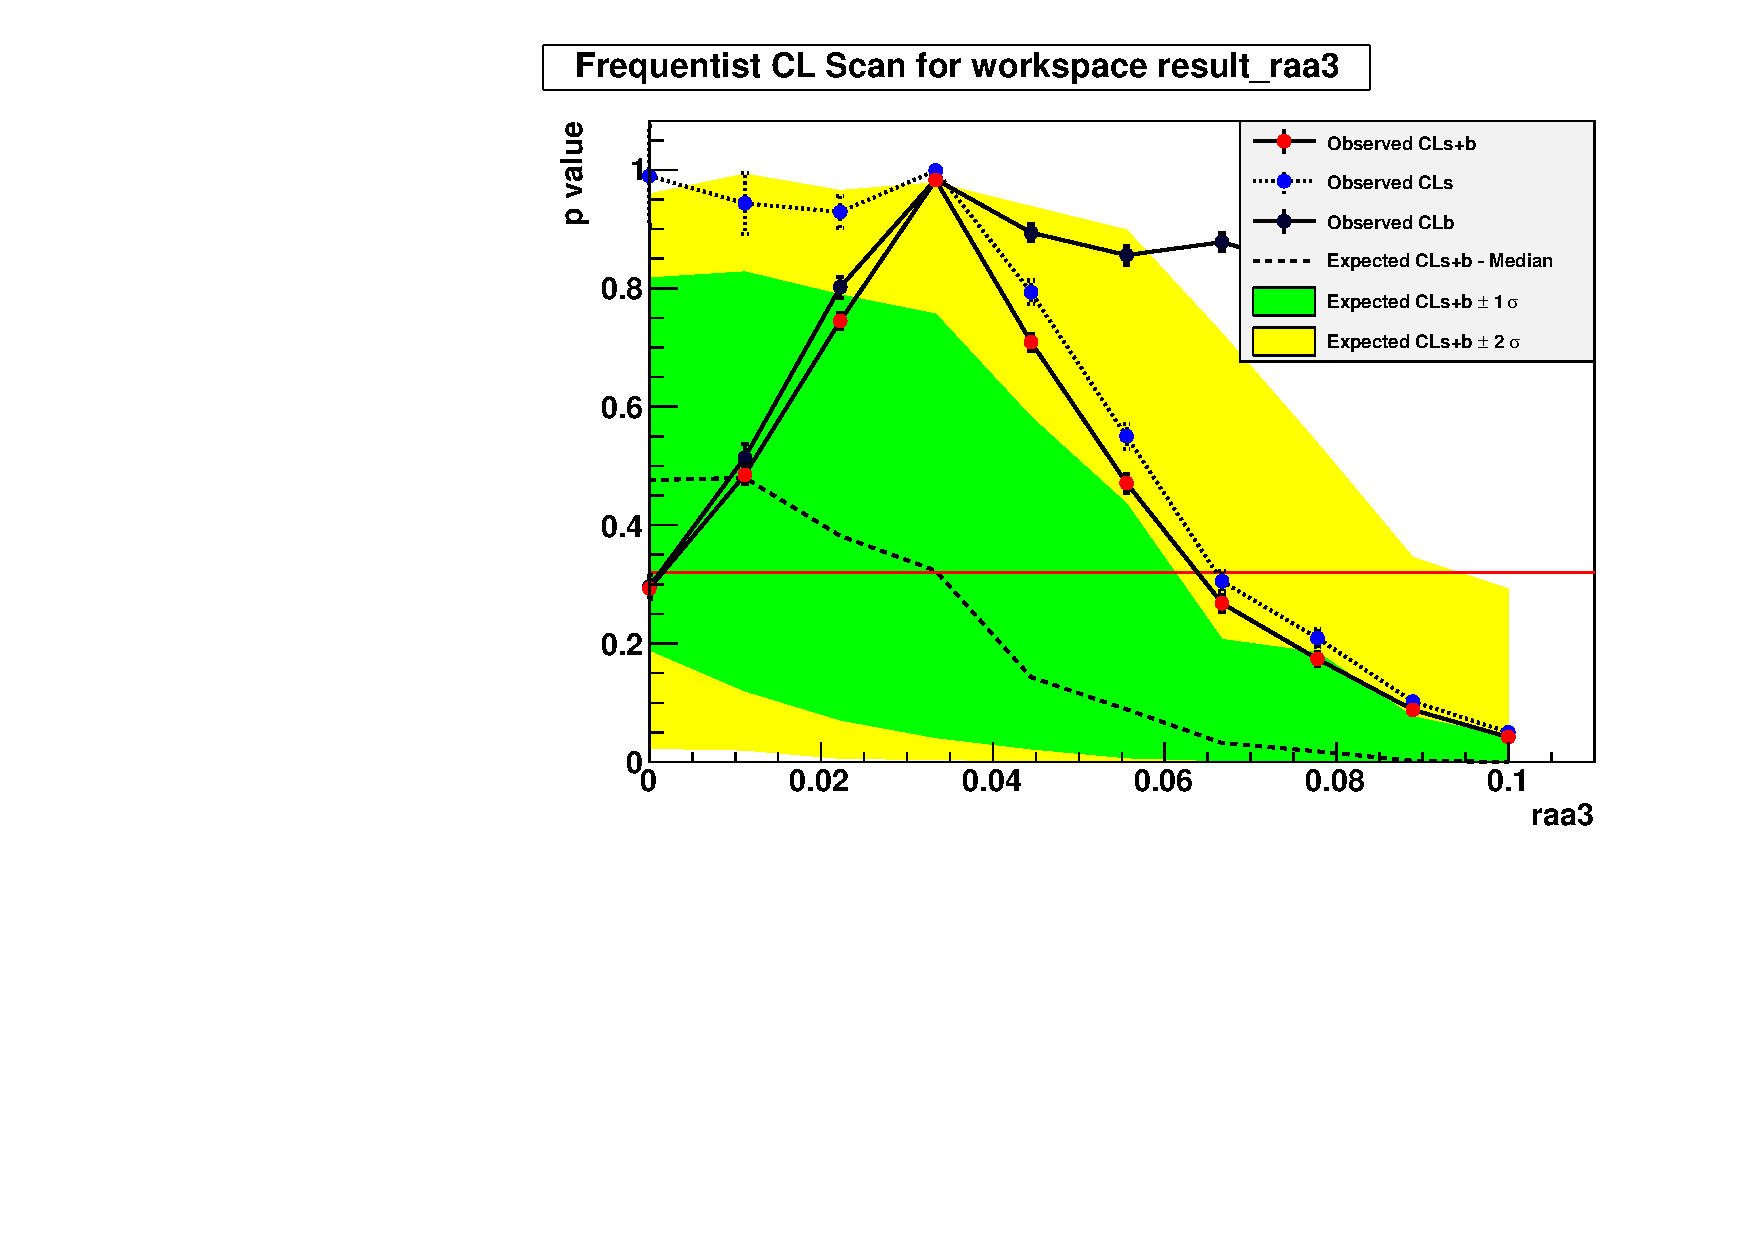
\includegraphics[angle=0,width=0.7\textwidth]{figures/limits/FCRaa3S_withsystematics68}\label{fig:/FC_Raa_Limit_MB_68}
%}\\
   \caption{$p$-value scan for $\raa(\PgUc)$ using the Feldman-Cousins technique at 68 \% confidence level.}
%A thousand pseudo experiments for each of the ten points scanned. Figs~\ref{fig:/FC_Raa_Limit_MB_68}:Observed $CL_s$; red curve, $H_{b}$ blue curve and black line is our Test Statistics.}
   \label{fig:FC_Raa_Limit_MB_68}
 \end{center}
\end{figure}




